%%%%%%%%%%%%%%%%%%%%%%%%%%%%%%%%%%%%%%%%%%%%%%%%%%%%%%%%%%%%%%%%%%%%%%%%%%%%%%%%
%2345678901234567890123456789012345678901234567890123456789012345678901234567890
%        1         2         3         4         5         6         7         8
\documentclass[letterpaper, 10 pt, conference]{ieeeconf}  % Comment this line out
% if you need a4paper
%\documentclass[a4paper, 10pt, conference]{ieeeconf}      % Use this line for a4

\usepackage{float}
% paper
% uso paquete bookmark para tener bien los outlines.
\usepackage{bookmark}

% Configuro el idioma.
\usepackage[utf8]{inputenc} % Importante para mantener acentos.
\usepackage[spanish, activeacute]{babel} % Requiere: texlive-lang-spanish. Por primera vez hay que ejecutar: texconfig init> log

% Paquete para poder usar acentos en $$.
\usepackage{mathtools}
%\setmathfont{XITS math}

\usepackage{tikz}
\usetikzlibrary{shapes.misc, positioning, shapes.geometric, arrows.meta}

\usepackage{siunitx}

% package to get \url
\usepackage{hyperref}
\hypersetup{
  colorlinks=true,
  linkcolor=magenta,
  filecolor=magenta,
  citecolor=magenta,      
  urlcolor=magenta,
}

% Graficos electrónicos
\usepackage{circuitikz}

\IEEEoverridecommandlockouts                              % This command is only
% needed if you want to
% use the \thanks command
\overrideIEEEmargins
% See the \addtolength command later in the file to balance the column lengths
% on the last page of the document

\usepackage{graphicx}
\usepackage{graphics}

% styling for matlab/octave code.
\usepackage{matlab-prettifier}
% Configuracion, con esto puede agregar ñ.
\lstset{
  literate={ñ}{{\~n}}1
}

% The following packages can be found on http:\\www.ctan.org
%\usepackage{graphics} % for pdf, bitmapped graphics files
%\usepackage{epsfig} % for postscript graphics files
%\usepackage{mathptmx} % assumes new font selection scheme installed
%\usepackage{times} % assumes new font selection scheme installed
\usepackage{amsmath} % assumes amsmath package installed
%\usepackage{amssymb}  % assumes amsmath package installed

\title{\LARGE \bf Laboratorio N° 4}

\author{
  Tom\'as Vidal\\
  {\it Circuitos Electrónicos 1}\\
  {\it Facultad de Ingenier\'ia, UNLP, La Plata, Argentina.}\\
  {\it 20 de Julio, 2024.}
}                                            % <-this % stops a space


% comienzo

% INTRO

% Figura
\newcommand{\image}[2] {
  \begin{figure}[H]
    \centering
    \includegraphics[width=0.43\textwidth]{./#1.png}
    \caption{#2}
    \label{fig:#1}
  \end{figure}
}

% Codigo
% \begin{lstlisting}[style=Matlab-editor]
% % el código va aca
% dispc("HELLO WORLD");
% \end{lstlisting}

\begin{document}
\maketitle
\thispagestyle{empty}
\pagestyle{empty}

\section{Introducción}
Se resuelven de manera analítica las consignas presentadas en el laboratorio 5 de circuitos electrónicos I; posteriormente se muestran los resultados de las mediciones hechas del mismo y las conclusiones.

\section{Topologías}
A partir del circuito presentado se pueden diferenciar 4 topologías diferentes, al cambiar j1, j2 y j3 de posición. A continuación se analizan con el método de bisección, ya que el circuito dado presenta un eje de simetría, y con este método el análisis es más sencillo.

\begin{figure}[H]
 \centering
 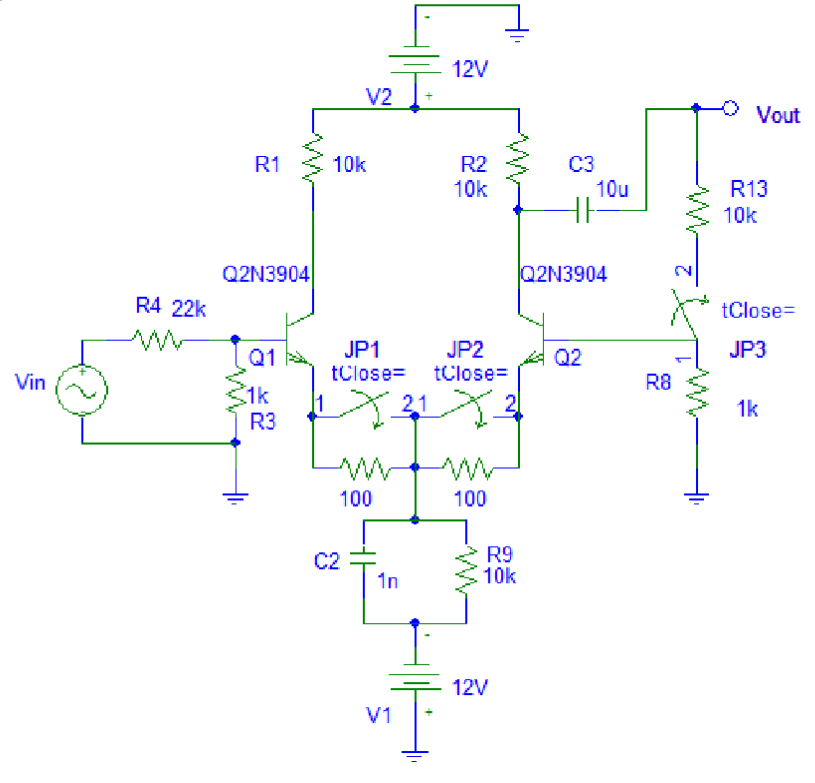
\includegraphics[width=0.43\textwidth]{./Imagenes/circuito_presentado.png}
 \caption{Circuito dado}
 \label{pic:circuito_presentado}
\end{figure}

\subsection{Topología 1}

\begin{figure}[H]
 \centering
 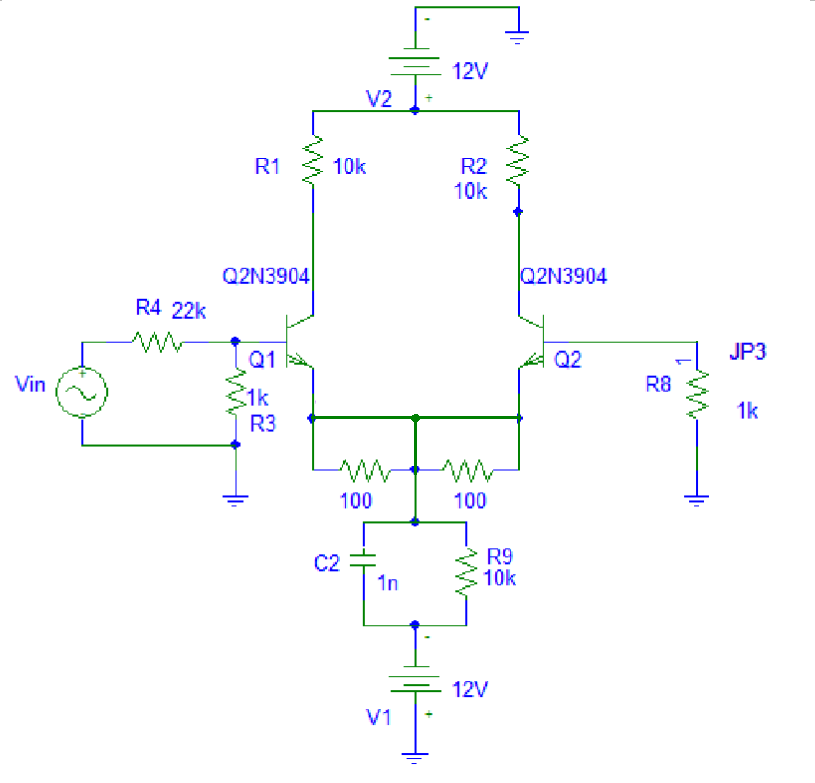
\includegraphics[width=0.43\textwidth]{./Imagenes/topologia1.png}
 \caption{Topología 1}
 \label{pic:topologia1}
\end{figure}

\begin{figure}[H]
 \centering
 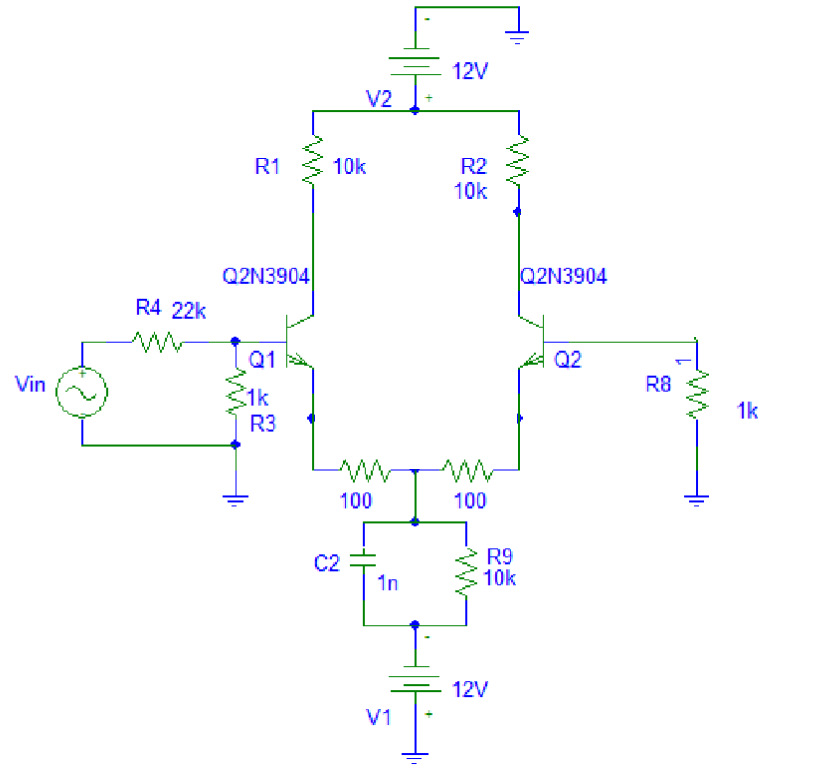
\includegraphics[width=0.43\textwidth]{./Imagenes/topologia2.png}
 \caption{Topología 2}
 \label{pic:topologia2}
\end{figure}

\begin{figure}[H]
 \centering
 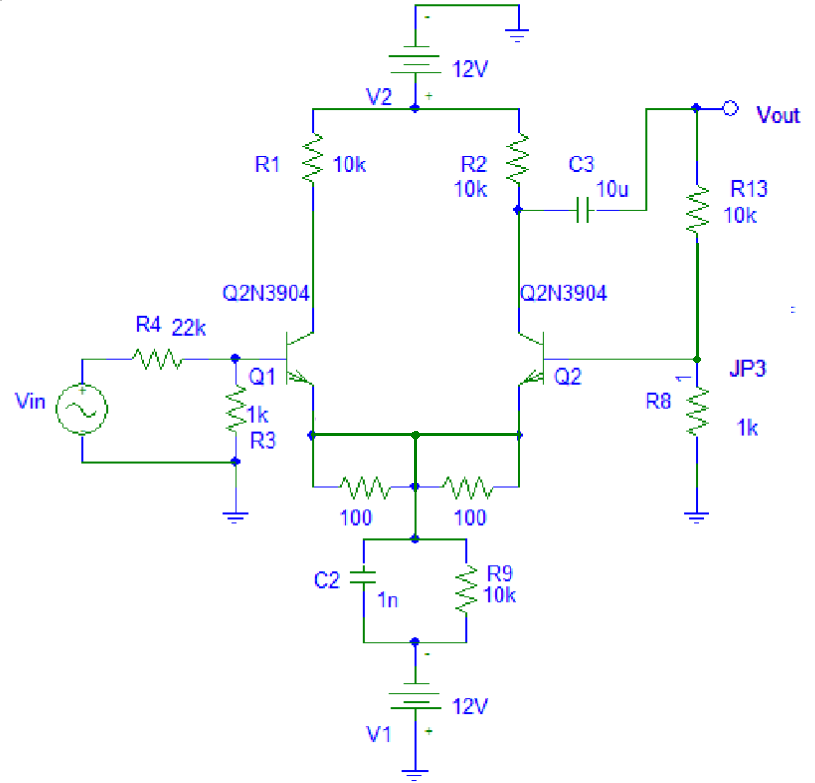
\includegraphics[width=0.43\textwidth]{./Imagenes/topologia3.png}
 \caption{Topología 3}
 \label{pic:topologia3}
\end{figure}

\begin{figure}[H]
 \centering
 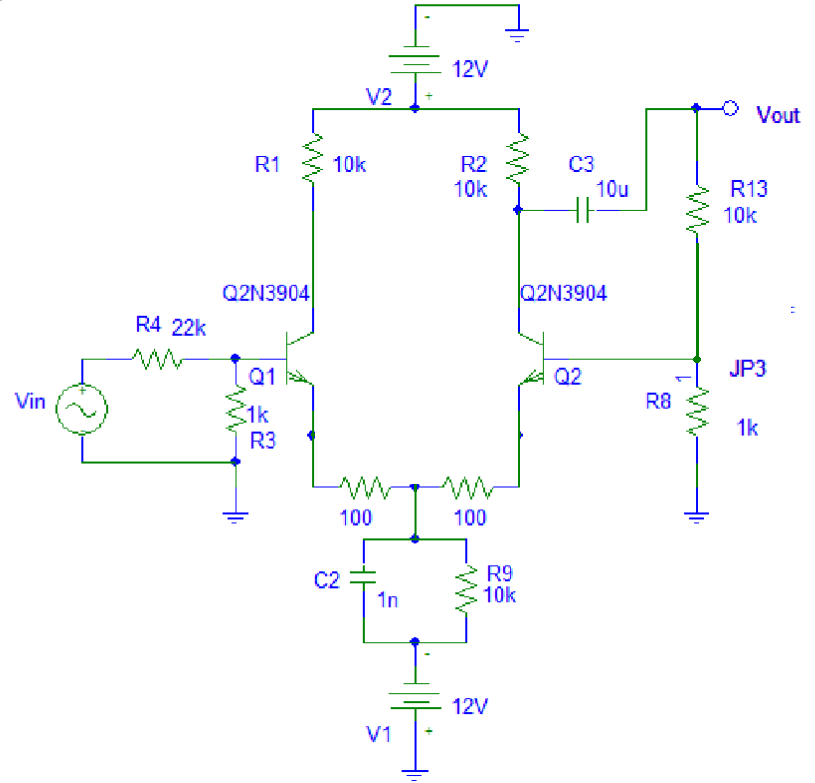
\includegraphics[width=0.43\textwidth]{./Imagenes/topologia4.png}
 \caption{Topología 4}
 \label{pic:topologia4}
\end{figure}

\end{document}
